%!TEX root = ../thesis.tex
%*******************************************************************************
%******************************* Introduction **********************************
%*******************************************************************************

\ifsetDraft
\else
    \cleartoevenpage
    \backgroundsetup{
        scale=1,
        color=black,
        opacity=1,
        placement=top,
        angle=0,
        contents={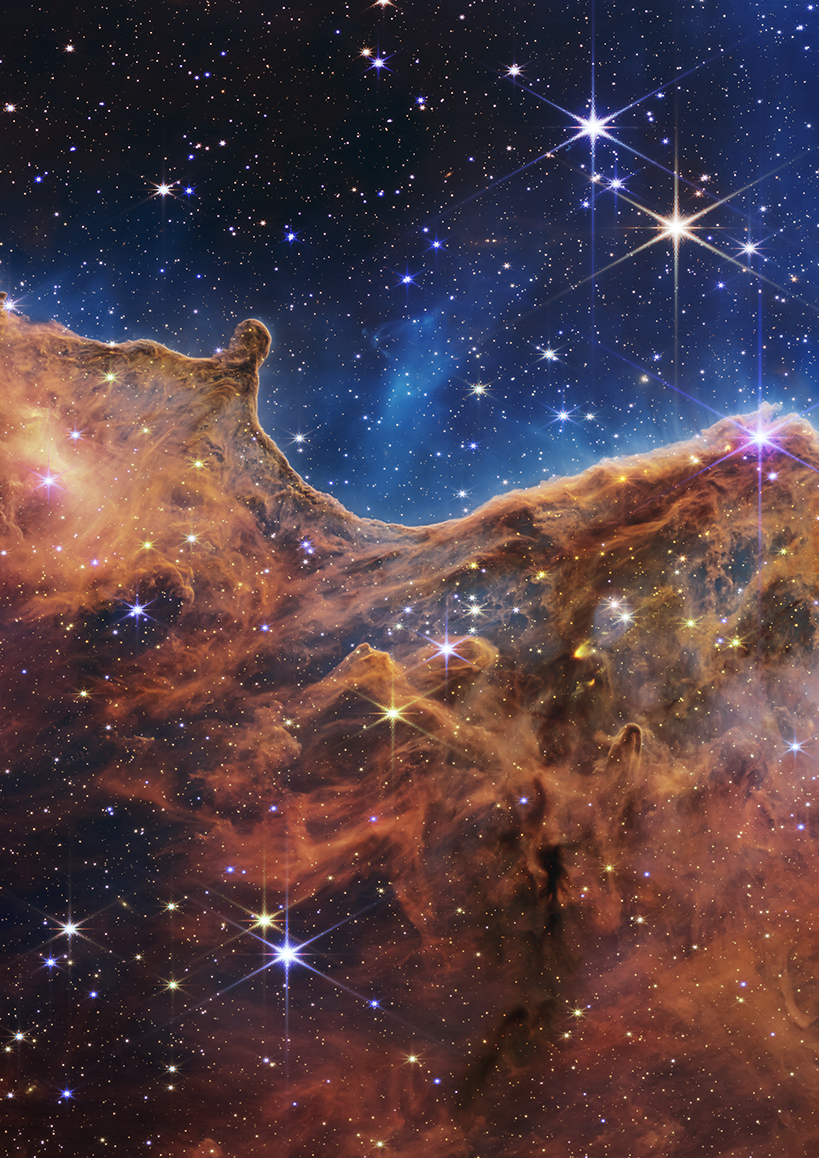
\includegraphics[width=\paperwidth]{Images/Carina_nebula_JWST1}}
    }
    \BgThispage
    
    \fancyfoot[C]{\color{white}\thepage}
    \fancyfoot[L]{\vspace{3.5ex}\tiny\textcolor{white}{Credit: NASA, ESA, CSA, STScI}}
    \clearpage
    \newpage
    
    \renewcommand{\CurrentTitleColor}{\color{white}}
\fi

\chapter{Conclusions and outlook}
\label{ch:Conclusions_and_outlook}

\ifsetDraft
\else
    \renewcommand{\CurrentTitleColor}{\color{black}}
    
    \vspace*{\fill}
    \setlength{\epigraphwidth}{0.6\textwidth}
    {\color{white} \epigraph{\textit{The Road goes ever on and on\\
                \hspace{2ex} Down from the door where it began.\\
                Now far ahead the Road has gone,\\
                \hspace{2ex} And I must follow, if I can,\\
                Pursuing it with eager feet,\\
                \hspace{2ex} Until it joins some larger way\\
                Where many paths and errands meet.\\
                \hspace{2ex} And whither then? I cannot say.}}{--- J.R.R. Tolkien, The Fellowship of the Ring (1954)}}
    \vspace*{\fill}
    
    \backgroundsetup{
        scale=1,
        color=black,
        opacity=1,
        placement=top,
        angle=0,
        contents={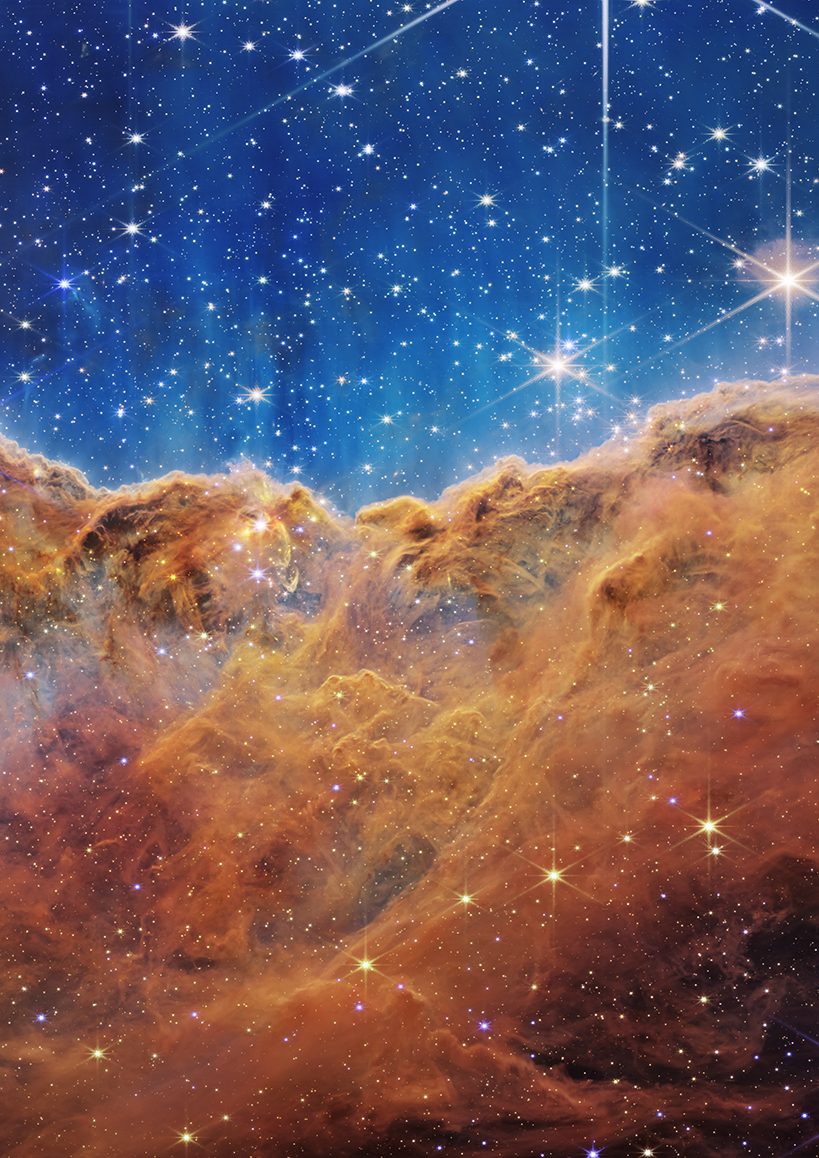
\includegraphics[width=\paperwidth]{Images/Carina_nebula_JWST2}}
    }
    \BgThispage
    
    \fancyhf{}
    \fancyfoot[C]{\color{white}\thepage}
    \newpage
    \setFancyHdr
\fi

\lettrine{I}{n the previous chapters}, I have discussed the properties of star-forming galaxies and the intergalactic medium in the early Universe. In this chapter, I briefly identify the main findings and potential directions of future investigations concerning the topics discussed.

\section{Conclusions}
\label{chCsec:Conclusions}

The main themes of this thesis revolve around galaxies in the early Universe and their large-scale environment, the cosmic web. In \cref{ch:Prospects_for_observing_the_low-density_cosmic_web_in_Lya_emission}, we discussed the potential of the \lya\ line to observe the diffuse, low-density IGM. Although challenging, the current and certainly the next generation of telescopes should be able to begin probing this largely unexplored territory in the post-reionisation Universe, complementary to 21-cm studies of neutral hydrogen in the dark ages and at cosmic dawn.

Meanwhile, the last decade has seen \textit{HST} extend the high-redshift galaxy frontier by identifying significant samples of galaxies in the very early Universe, towards the end of, and indeed in the heart of, the reionisation epoch. At the same time, ground-based spectrographs have been pushed to their limits to spectroscopically follow up these intrinsically faint distant galaxies, as exemplified in \cref{ch:Assessing_the_sources_of_reionisation}. In this chapter, we conducted a case study of what we expect might be a typical EoR galaxy, in preparation for the NIR spectroscopy of galaxies well and truly inside the EoR that will be undertaken by \textit{JWST}. We explored several promising emission-line diagnostics, finding tentative evidence for LyC escape and a departure from the FMR. Though this is in line with expectations for a young, metal-poor galaxy, we still lack convincing evidence that these effects are commonplace among EoR galaxies due to the observational challenges faced in spectroscopy of high-redshift galaxies, many of which however may soon be overcome by \textit{JWST} (see \cref{chCssec:JWST}).

\Cref{ch:Dual_constraints_with_ALMA} discussed how ALMA has proven to be a critical tool for studying the ISM properties of high-redshift galaxies in the FIR regime. As expected, these systems appear to have young stellar populations and hard radiation fields. However, somewhat surprisingly, we also found indications that some of these galaxies may have already reached quite advanced evolutionary stages, having already built up significant amounts of metals and dust.

Naturally, a lot of open questions still remain in spite of -- but in many cases also provoked by -- the findings of spectroscopic studies that have been performed to date by the astronomical community focussing on the early Universe. In the next section, I will discuss some of the potential avenues for the continuation of the research presented in this thesis in light of two of the main facilities expected to be at the cutting edge of high-redshift extragalactic science over the next few years, \textit{JWST} and ALMA.

\section{Outlook}
\label{chCsec:Outlook}

\subsection{Prospects for extragalactic science with \textit{JWST}}
\label{chCssec:JWST}

In \cref{ch:Assessing_the_sources_of_reionisation,ch:Dual_constraints_with_ALMA}, I have discussed how spectroscopic measurements of high-redshift galaxies are starting to characterise the process of star formation in the early Universe and its contribution to Cosmic Reionisation. Importantly, the recent commissioning of \textit{JWST} \citep{2006SSRv..123..485G} will enable detailed rest-frame UV and optical spectroscopic (and photometric) measurements in statistically meaningful samples of EoR galaxies. In the following, I briefly describe the capabilities of the four different instruments on board \textit{JWST} and their observing modes relevant to the topics covered here.

Already briefly discussed in \cref{ch:Assessing_the_sources_of_reionisation}, NIRSpec \citep{2022A&A...661A..80J, 2022A&A...661A..81F} is capable of multi-object, fixed-slit, and IFU spectroscopy in the NIR regime ($0.6$-$5.3 \, \mathrm{\upmu m}$) at three different spectral resolution modes: low ($R \approx 100$), medium ($R \approx 1000$), and ``high'' ($R \approx 2700$) resolution. The Near-Infrared Camera \citep[NIRCam;][]{2005SPIE.5904....1R, 2012SPIE.8442E..2NB} contains two nearly identical modules covering adjacent fields of view and operates in approximately the same wavelength regime as NIRSpec ($0.6$-$5 \, \mathrm{\upmu m}$). A dichroid allows both modules to simultaneously image the same field in a short-wavelength ($0.6$-$2.3 \, \mathrm{\upmu m}$) and long-wavelength ($2.4$-$5 \, \mathrm{\upmu m}$) channel, the latter of which is also used to perform wide-field slitless spectroscopy at medium resolution ($R \approx 1400$). The Near-Infrared Imager and Slitless Spectrograph \citep[NIRISS;][]{2012SPIE.8442E..2RD} provides complementary wide-field slitless spectroscopy at short wavelengths ($0.8$-$2.2 \, \mathrm{\upmu m}$) as well as NIR imaging ($0.8$-$5 \, \mathrm{\upmu m}$). Finally, the Mid-Infrared Instrument \citep[MIRI;][]{2015PASP..127..584R} has an imaging mode with a number of broadband MIR filters ($4.9$-$28.8 \, \mathrm{\upmu m}$), but it is also capable of low-resolution ($R \approx 100$) fixed-slit spectroscopy and medium-resolution ($R \approx 2500$) IFU spectroscopy.

One of the main deep, extragalactic surveys that \textit{JWST} will carry out is JADES, the \textit{JWST} Advanced Extragalactic Survey \citep[e.g.][]{2018ApJS..236...33W}, exploiting the combined capabilities of the NIRSpec and NIRCam instruments. The wealth of spectroscopic data it will obtain as a follow-up of high-redshift targets identified in photometric data taken by \textit{HST}, and \textit{JWST}/NIRCam in the second stage of the survey, will allow a wide range of science goals relating to galaxies in the early Universe to be explored.

First of all, the imaging from NIRCam (and MIRI, if available), combined with the low-resolution NIRSpec spectra, will probe the stellar continuum not only of the very young, but also more mature stellar populations (cf. \cref{chIsssec:Counting_stars,chIssec:Stellar_continuum}), thereby significantly improving the accuracy of stellar mass estimates compared to current constraints derived from shorter wavelengths that are dominated by young stellar light \citep[e.g.][]{2022arXiv220803281T}. Concerning the spectroscopy specifically, JADES is expected to detect a significant number of high-redshift ($z \gtrsim 6$) \lya\ emitters, whose prevalence as a function of redshift, owing to the effect of IGM absorption discussed in \cref{chIsssec:Cosmic_Reionisation}, can be used to study the cosmic neutral fraction in the later stages of Cosmic Reionisation \citep{2010MNRAS.408.1628S, 2014ApJ...793..113P, 2014MNRAS.443.2831C, 2018ApJ...856....2M, 2019MNRAS.489.2669M, 2022MNRAS.512.5960M}. In combination with rest-frame UV and optical emission lines and continuum, the expected ionising photon production and escape of these systems can be characterised, among many other physical properties. In particular, the low-resolution ($R \approx 100$) mode will be used to study the continuum emission to constrain stellar masses and ages, while the medium-resolution ($R \approx 1000$ and $R \approx 2700$) gratings will deliver spectra suitable for detailed emission-line studies. For instance, traditional methods using strong lines in the rest-frame optical (e.g. \Halpha\ and $\OIIIf \, \lambda \, 5008 \, \Angstrom$) can for the first time be applied to EoR galaxies to measure SFRs and metallicities (cf. \cref{chIssec:Chemical_enrichment}), characterise AGN activity \citep[\cref{chIssec:Nebular_emission_and_emission-line_diagnostics}; see also][]{2022arXiv220807467B}, and study the kinematics (using the higher-resolution mode, $R \approx 2700$). The \lya\ line profile can be used to map out the structure of ionised regions carved out by galaxies \citep[``ionised bubbles'';][]{2020MNRAS.499.1395M}. In the absence of \lya\ emission, different diagnostics of LyC escape (such as the $\MgII \, \lambda \, 2796, 2804 \, \Angstrom$ doublet) can be applied to establish a census of star-forming galaxies actively contributing to reionisation. Last, but certainly not least, there are many aspects that are impossible to forecast: for instance, \textit{JWST} may be able to find evidence for Population-III stars \citep[e.g.][]{2022MNRAS.513.5134N}, in addition to many other unexpected discoveries.

\subsection{Prospects for extragalactic science with ALMA}
\label{chCssec:ALMA}

As emphasised in \cref{ch:Dual_constraints_with_ALMA}, the presence of dust in EoR galaxies may be significant. The dust properties, however, are still largely unconstrained: in particular, the uncertainty in the dust temperature has a large impact on many derived physical properties such as the dust mass and obscured SFR (\cref{chDsec:Discussion:Dust_properties}). Therefore, it is crucial to study the FIR SED at multiple wavelengths and begin to establish the typical dust properties of EoR galaxies. Preliminary efforts using the \program{mercurius} code to empirically constrain the greybody parameters of all high-redshift galaxies with multi-band dust-continuum detections point out that while some galaxies host substantial dust reservoirs -- perhaps more than would be expected as a result of SN activity alone -- there does not seem to be a strong redshift evolution in the dust emissivity \citetext{Witstok et al., in prep.}.

In addition, to better understand the emergence of these dust reservoirs, we have an approved ALMA program in Cycle 9 (2022.1.00925.S; PI: Witstok) that will constrain the dust properties of COS-3018555981 (discussed in detail in \cref{chDsec:Discussion:Dust_properties}) with observations in bands 5, 7, and 8. With several dust-continuum detections, we can infer a first estimate of the shape of its FIR SED which will allow us to more accurately measure the greybody parameters (i.e. dust temperature, mass, and emissivity). As shown in \cref{ch:Dual_constraints_with_ALMA}, this will potentially reveal the existence of cold, massive dust reservoir in the very early Universe, in stark contrast to what may be expected of typical young star-forming galaxies at this era \citep{2022MNRAS.513.3122S, 2022MNRAS.tmpL..72V}. Although it will merely be a singular, perhaps extreme example, such a detailed dissection of the dust emission of a normal star-forming galaxy in the EoR is a crucial first step towards the characterisation of dust properties at high redshift.

This program will simultaneously cover the \NII\ 122 $\upmu\mathrm{{m}}$ line, which (even if it remains undetected) can be used in combination with \OIIILam\ to probe hardness of the radiation field and constrain the ionisation parameter. This highlights one possible ways where ALMA and \textit{JWST} (with measurements of e.g. \Halpha\ and $\OIIIf \, \lambda \, 5008 \, \Angstrom$) can paint a physical picture together through a combination of multi-wavelength observations of the ionised gas. ALMA is able to complement this picture further with measurements not only of the cold dust component, but perhaps soon also of cold gas, for instance with the advent of band-1 receivers.

It is uncertain what surprises will be revealed in relation to the emergence of the first galaxies in the coming years by ALMA, \textit{JWST}, and other facilities. Above all, however, it is clear that the outlook for extragalactic astronomy is exceptionally bright.